\documentclass[a4paper,12pt]{report}
\usepackage{graphicx} 		% images
\usepackage[utf8]{inputenc}	% encoding: UTF-8
\usepackage[italian]{babel}	% language
\usepackage[margin=0.5in, includefoot]{geometry}	% margin
\usepackage{scrextend}		% KOMA scripts?
\usepackage{array}			% table width
\usepackage[table]{xcolor}	% table colors
\usepackage{tocloft}			% table of contents
\usepackage{hyperref}			% hyperlinks inside document
\usepackage[italian]{cleveref}	% ^

\renewcommand{\cftsecleader}{\cftdotfill{\cftdotsep}}
\newcommand\chap[1]{
    \chapter*{#1}
    \addcontentsline{toc}{chapter}{#1}
    \markboth{#1}{#1}}
    
\newcommand\sect[1]{
    \section*{#1}
    \addcontentsline{toc}{section}{#1}
    \markboth{#1}{#1}}

\title{
\Huge \textbf{Elaborato per il corso di Basi di Dati} \\
[4mm]
\large A.A. 2020/2021 \\
\large Progetto di una base di dati per la gestione di un servizio online
}
\author{Christian Ricci \\
christian.ricci3@studio.unibo.it \\
0000915693}

\begin{document}

\maketitle
\tableofcontents

\chap{Analisi dei requisiti}

Si vuole realizzare un database per gestire un servizio online di videogiochi. Il database dovrà immagazzinare dati relativi ai videogiochi, agli utenti, alle iscrizioni. Gli utenti potranno {giocare} accedendo al servizio e potranno partecipare in sessioni multiplayer. I direttori del servizio potranno aggiungere nuovi videogiochi, consultare statistiche riguardanti gli utenti, etc.

\sect{Definizione delle specifiche in linguaggio naturale}

Il testo ottenuto dall'intervista con l'azienda è il seguente:\\\\

\begin{addmargin}[4em]{4em}
La casa produttrice di videogiochi GameSoft vuole realizzare un servizio online per tutti i videogiochi che ha pubblicato in passato. Gli utenti che si registreranno a questo nuovo servizio potranno accedere ad un catalogo di videogiochi e potranno giocare liberamente a qualunque gioco nel catalogo senza ulteriori costi. Degli utenti si vuole tener traccia del nome utente, della password, dell'email, dell'età e anche di un numero di telefono. Il numero di telefono è opzionale e un utente lo può dare anche dopo essersi registrato.

Al momento della registrazione l'utente potrà scegliere tra tre piani: il primo prevede un periodo gratuito di un mese, che non si potrà rinnovare; a quel punto l'utente deve decidere tra gli altri due piani. Il secondo piano prevede un costo e comporta l'iscrizione al servizio per un mese. Il terzo piano, invece, comporta l'iscrizione per un anno. Si vuole anche memorizzare lo storico delle iscrizioni per ogni utente.

Per ogni videogioco si vuole memorizzare il titolo, il genere, l'anno di rilascio, l'azienda sviluppatrice e il produttore esecutivo. Per ogni utente del servizio si vuole anche dare la possibilità di acquistare una copia fisica di qualunque videogioco, che, però, potrebbe anche non essere disponibile. Ogni videogioco ha un prezzo fisso per la copia. Si vuole anche memorizzare lo storico degli acquisti per ogni utente.

Per ogni utente si vuole anche memorizzare alcune particolare statistiche: il numero di ore trascorso su un videogioco, il numero di ore trascorse in totale a giocare, una lista dei giochi più giocati, una lista dei giochi preferiti (a scelta dell'utente). Queste statistiche potranno essere viste dai direttori del servizio.

Infine, si vuole anche immagazzinare anche alcune informazioni relative al multiplayer. Gli utenti del servizio possono iniziare una sessione di gioco con altri utenti e scegliere un videogioco da giocare: si vuole memorizzare i dati di ogni sessione, che includeranno gli utenti partecipanti, il videogioco scelto e altre statistiche quali il tempo trascorso. Si vuole anche mantenere uno storico delle sessioni per ogni utente. Ovviamente, si dovrebbe tener conto che il gioco scelto sia effettivamente un gioco multiplayer. \\\\

\end{addmargin}

\sect{Estrazione dei concetti fondamentali}

I concetti principali sono riassunti in questa tabella.

\renewcommand{\arraystretch}{1.8}
\arrayrulecolor[HTML]{a7acb1}
\begin{table}[h!]
\begin{center}
	\begin{tabular}{ m{6cm} m{6cm} m{6cm} }
	\rowcolor[HTML]{deecdc}
	\textbf{Termine} & \textbf{Breve descrizione} & \textbf{Eventuali sinonimi} \\
	Utente & Colui che accede al servizio e interagisce con i giochi presenti. & Nessuno \\
	\hline
	Videogioco & TODO & TODO \\
	\hline
	Piano & TODO & Abbonamento \\
	\hline
	Copia Videogioco & TODO & Copia \\
	\hline
	Statistiche & TODO & TODO \\
	\hline
	Sessione di gioco & TODO & Sessione, \\
	\hline
	\end{tabular}
\end{center}
\caption{La tabella dei concetti principali.}
\end{table}

A seguito della lettura e comprensione dei requisiti richiesti dal cliente, si procede sviluppando un testo che
ne riassuma tutti i concetti e in particolare ne estragga quelli principali, risultando essere in questo modo
meglio fruibile per la realizzazione della base di dati.\\\\

\begin{addmargin}[4em]{4em}
Per ogni \textbf{\textit{utente}} si memorizza nome, cognome, password, email, età e opzionalmente numero di telefono. Ogni utente deve avere un codice univoco, fornito al momento della registrazione.

Un utente può stipulare più \textbf{\textit{piani}}: un piano gratuito è attivato al momento della registrazione. Per ogni tipo di piano c'è una durata e un prezzo e ogni piano viene mantenuto in uno storico, in cui si memorizza anche la data d'inizio (non c'è bisogno della data di scadenza, dato che si può evincere dal tipo di piano). Ogni utente può avere un solo piano attivo alla volta.

Per ogni \textbf{\textit{videogioco}} si deve memorizzare titolo, genere, anno di rilascio, azienda sviluppatrice e produttore esecutivo. Si devono anche memorizzare prezzo e quantità di copie per ogni videogioco. Per ogni copia, invece, si deve memorizzare la data di acquisto.

Occorre memorizzare le \textbf{\textit{statistiche}} per ogni coppia utente-videogioco e per ogni coppia si memorizzano le ore giocate. Non occorre memorizzare statistiche come la lista dei giochi più giocati: queste possono essere trovate partendo da altri attributi.

Infine, per ogni \textbf{\textit{sessione}} occorre memorizzare gli utenti partecipanti e il gioco scelto. Dato che non tutti i giochi permettono di giocare in multiplayer, bisogna fare una distinzione tra \textbf{\textit{gioco single player}} e \textbf{\textit{gioco multiplayer}}. Si suppone, inoltre, che un videogioco multiplayer abbia un numero minimo e massimo di giocatori. \\\\

\end{addmargin}

Da questo testo si può anche evincere le principali azioni richieste:

\begin{itemize}
\item Registrazione di un utente;
\item Sottoscrittura di un tipo di piano da parte di un utente;
\item Visualizzazione dei piani da parte di utente;
\item Visualizzazione dei giochi disponibili nel catalogo;
\item Acquisto di una copia di un videogioco;
\item Visualizzazione di un profilo utente, con tutte le relative statistiche;
\item Visualizzazione di dati specifici per un videogioco;
\item Creazione di nuove sessioni di gioco da parte di un utente;
\item Partecipazione di un utente ad una sessione di gioco;
\end{itemize}

\chap{Progetto dello schema concettuale}

La strategia adottata per creare lo schema concettuale è una strategia mista, orientata al bottom-up. Il database è composto da più ambiti, che verranno analizzati e raffinati uno ad uno, per poi creare uno schema finale che comprenda tutto il database.

\sect{Schema scheletro}

L'associazione tra utente e piano è abbastanza evidente. Per rappresentare i tre tipi di piano, si è scelto di usare specializzazioni per la più generica entità piano. Per rappresentare lo storico dei piani, si è deciso di fare una reificazione dell'associazione tra utente e piano: quest'entità conterrà inoltre la data di inizio. La data di scadenza di un piano non deve necessariamente essere memorizzata, dato che si può evincere subito dal tipo di piano. Per identificare le varie entità, si è scelto di identificare sia utenti che piani con un ID unico, mentre le stipulazioni sono identificate dall'utente, dal piano e dalla data di inizio. Un'utente non può stipulare un piano se ha già un piano in corso: questo vincolo non si può esprimere con facilità nello schema concettuale, perciò sarà inserito come business rule.

\begin{figure}[h]
\centering{}
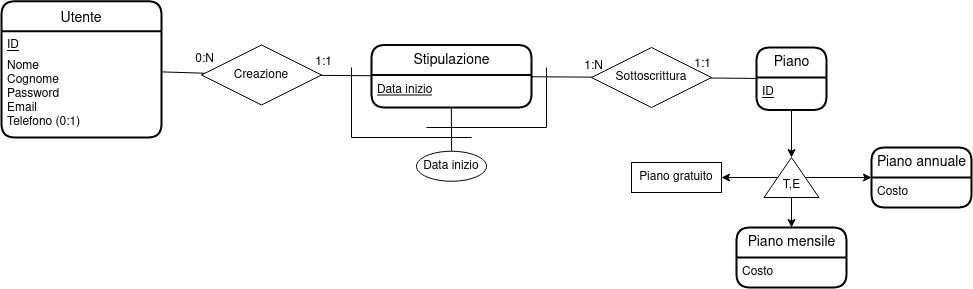
\includegraphics[width=\textwidth]{piani.png}
\caption{Lo schema Entity-Relationship relativo at utenti e piani.}
\label{img:schema_piano}
\end{figure}

Riguardo alle relazioni tra Utente e Videogioco, abbiamo sia una relazione che riguarda le statistiche, sia una che riguarda l'acquisto di copie fisiche di un videogioco da parte dell'utente. Dato che occorre immagazzinare le statistiche riguardo coppie utente-videogioco, l'associazione statistiche viene convertita in entità. Questa entità riguarda i singoli videogiochi: per ottenere statistiche quali i giochi preferiti di un utente basterà creare una query a lato software. L'entità statistiche è identificata tramite l'utente e il videogioco in questione.

La conversione a entità accade anche per Copia Videogioco, dato che per un videogioco ci possono essere più copie fisiche. Il prezzo di ogni copia non riguarda le singole copie, bensì riguarda il gioco in sè, e si suppone inoltre che questo dato rimanga costante nel tempo, per cui è stato messo come attributo di videogioco. Una copia può anche rimanere invenduta, quindi si è pensato di immagazzinare il dato relativo alla data di acquisto come attributo dell'associazione Acquisto. Ogni copia è identificata tramite un codice univoco e l'associazione al videogioco di cui è copia.

\begin{figure}[h]
\centering{}
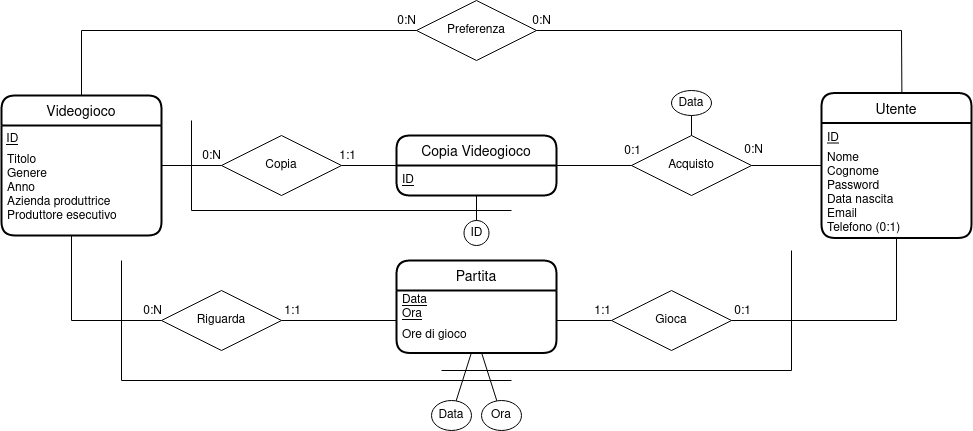
\includegraphics[width=\textwidth]{vg.png}
\caption{Lo schema Entity-Relationship relativo agli utenti, videogiochi, copie e statistiche.}
\label{img:schema_vg}
\end{figure}

L'ambito relativo alle sessioni di gioco multiplayer è il più semplice. Un Videogioco Multiplayer è una specializzazione di Videogioco ed aggiunge gli attributi di numero minimo e massimo di giocatori. Le due entità Utente e Videogioco Multiplayer sono associate all'entità Sessione, che raccoglie dati relativi alla specifica sessione. Una sessione è identificata dall'attributo ID di Sessione e dall'associazione con Videogioco Multiplayer. Per sottolineare il fatto che un solo utente può dare inizio ad una sessione, mentre più utenti possono parteciparvi, si è optato per due associazioni, Creazione e Partecipazione, tra Utente e Sessione. Rimane un vincolo inespresso: in una sessione, il numero minimo e massimo di giocatori dipende dal videogioco, cosa difficile da esprimere usando il modello ER.

\begin{figure}[h!]
\centering{}
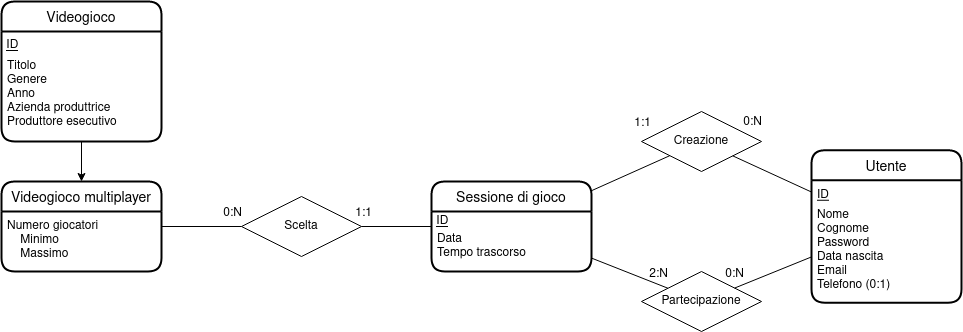
\includegraphics[width=\textwidth]{session.png}
\caption{Lo schema Entity-Relationship relativo alle sessioni.}
\label{img:schema_sessione}
\end{figure}

\section*{Schema finale}

\begin{figure}[h!]
\centering{}
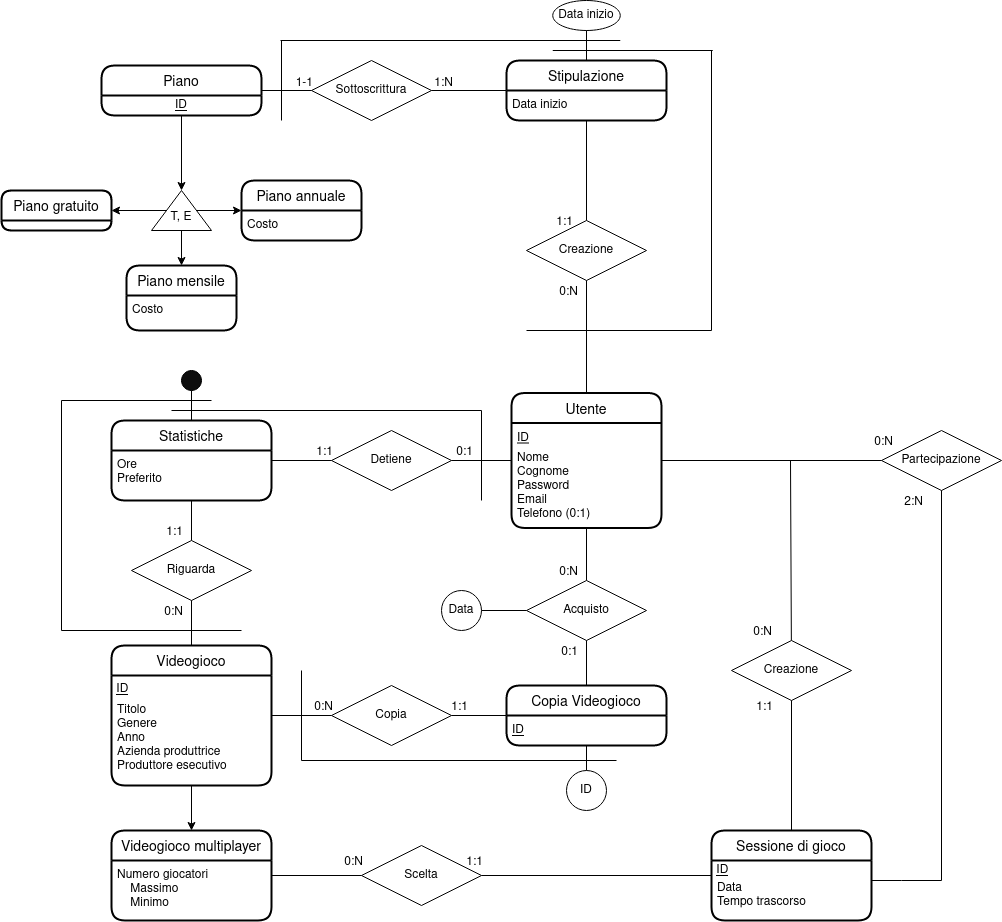
\includegraphics[width=\textwidth]{er.png}
\caption{Lo schema Entity-Relationship finale.}
\label{img:schema_sessione}
\end{figure}

\chap{Progettazione logica}

\sect{Stima del volume dei dati.}

\begin{table}[h!]
\begin{center}
	\begin{tabular}{ l l l }
	\rowcolor[HTML]{deecdc}
	\textbf{Concetto} & \textbf{Costrutto} & \textbf{Volume} \\
	Utente & E & 10.000 \\
	Videogioco & E & 1000 \\
	\hline
	\end{tabular}
\end{center}
\caption{La tabella dei volumi.}
\end{table}

\sect{Descrizione delle operazioni principali e stima della loro frequenza}

\begin{table}[h!]
\begin{center}
	\begin{tabular}{ l l }
	\rowcolor[HTML]{deecdc}
	\textbf{Operazione} & \textbf{Frequenza} \\
	Giocare ai videogiochi & 10000 al giorno \\
	\hline
	\end{tabular}
\end{center}
\caption{La tabella dei volumi.}
\end{table}

\sect{Schemi di navigazione e tabelle degli accessi}

\begin{table}[h!]
\begin{center}
	\begin{tabular}{ l l l l }
	\rowcolor[HTML]{deecdc}
	\textbf{Concetto} & \textbf{Costrutto} & \textbf{Accessi} & \textbf{Tipo} \\
	Utente & E & 1 & S \\
	\hline
	\end{tabular}
\end{center}
\end{table}

\sect{Raffinamento dello schema}

\sect{Analisi delle ridondanze}

\sect{Traduzione di entità e associazioni in relazioni}

\sect{Schema relazionale finale}

\sect{Costruzione delle tabelle in linguaggio SQL}

\sect{Traduzione delle operazioni in query SQL}

\chap{Progettazione dell'applicazione}

\sect{Descrizione dell'architettura dell'applicazione}

\end{document}